\chapter{TỔNG QUAN}
\label{Chapter2}

Bài toán sinh cử chỉ cũng tương tự như các bài toán khác, đều đã nghiên cứu và phát triển song hành với các phương pháp học máy truyền thống và hiện đại. Gồm các nhóm phương pháp dựa trên luật và các phương pháp dựa trên dữ liệu.  Đầu tiên luận văn trình bày về các đặc điểm của cử chỉ \autoref{sec:relationspeechandgesture}, từ đó là tiền đề cho việc học mối quan hệ giữa cử chỉ, văn bản và giọng nói. Trong mục \autoref{sec:commonstage}, luận văn sẽ trình bày về các công đoạn chung trong các phương pháp sinh cử chỉ.
Ở phần \autoref{sec:relatedwork}, luận văn trình bày về các phương pháp đã được sử dụng trong quá trình sinh cử chỉ. Luận văn sẽ so sánh các phương pháp, từ đó nêu lý do luận văn sử dụng mô hình diffusion để áp dụng cho bài toán sinh cử chỉ.
Trong phần \autoref{sec:diffusionbase}, luận văn sẽ trình bày về cách các mô hình diffusion được áp dụng cho bài toán sinh cử chỉ gần đây.

\section{Đặc điểm của cử chỉ}
\label{sec:relationspeechandgesture}

Theo ngôn ngữ học, cử chỉ có thể được phân thành 6 nhóm chính: cử chỉ thích nghi (adaptors), cử chỉ biểu tượng (emblems), cử chỉ chỉ định (deictics), cử chỉ biểu trưng (iconics), cử chỉ ẩn dụ (metaphorics), và cử chỉ nhấn mạnh (beat) \cite{ekman1969repertoire}, \cite{sebeok2011advances}. Trong số đó, cử chỉ nhấn mạnh không mang ý nghĩa ngữ nghĩa trực tiếp nhưng đóng vai trò quan trọng trong việc đồng bộ nhịp điệu giữa giọng nói và cử chỉ \cite{kipp2005gesture}, \cite{sebeok2011advances}. Tuy nhiên, nhịp điệu giữa giọng nói và cử chỉ nhấn mạnh không hoàn toàn đồng bộ, khiến việc học mối quan hệ thời gian giữa chúng trở nên phức tạp \cite{mcclave1994gestural}, \cite{bhattacharya2021speech2affectivegestures}, \cite{kucherenko2020gesticulator}, \cite{yoon2020speech}.

Cử chỉ tương tác với các cấp độ thông tin khác nhau trong giọng nói \cite{sebeok2011advances}. Chẳng hạn, cử chỉ biểu tượng, như hành động giơ ngón cái, thường liên quan đến thông tin ngữ nghĩa cấp cao (ví dụ: "tốt" hoặc "tuyệt vời"), trong khi cử chỉ nhấn mạnh thường đi kèm với thông tin cấp thấp như nhấn mạnh trong âm thanh. Các nghiên cứu trước đây thường chỉ sử dụng đặc trưng từ lớp cuối cùng của bộ mã hóa giọng nói để sinh cử chỉ \cite{alexanderson2020style}, \cite{bhattacharya2021speech2affectivegestures}, \cite{kucherenko2021large}, \cite{qian2021speech}, \cite{yoon2022genea}. Tuy nhiên, cách tiếp cận này có thể làm trộn lẫn thông tin từ nhiều cấp độ, dẫn đến khó khăn trong việc phân tách rõ ràng nhịp điệu và ngữ nghĩa.

Như các nghiên cứu ngôn ngữ học chỉ ra \cite{kipp2005gesture}, \cite{neff2008gesture}, \cite{webb1997linguistic}, cử chỉ trong giao tiếp hàng ngày có thể được chia thành một số lượng giới hạn các đơn vị ngữ nghĩa với các biến thể chuyển động khác nhau. Dựa trên giả định này, được phân tách đặc trưng giọng nói thành hai loại: đặc trưng cấp cao đại diện cho các đơn vị ngữ nghĩa, và đặc trưng cấp thấp xác định các biến thể chuyển động. Từ đó, mối liên hệ giữa chúng được học thông qua các lớp khác nhau của bộ mã hóa giọng nói. Các thử nghiệm chứng minh rằng cơ chế này có khả năng tách biệt rõ ràng các đặc trưng ở nhiều cấp độ, đồng thời tổng hợp được cử chỉ phù hợp về ngữ nghĩa và phong cách.



\section{Tổng quan các phương pháp cho bài toán sinh cử chỉ}
\label{sec:relatedwork}

\subsection{Phương pháp dựa trên luật}

\subsubsection{Nguyên lý chung}

Dựa trên việc xây dựng các quy tắc hoặc luật rõ ràng, các quy tắc được định nghĩa thủ công, xác định cách hệ thống xử lý đầu vào để tạo ra đầu ra.

\subsubsection{Phương pháp}

Tiêu biểu cho phương pháp dựa trên luật là \textit{Robot behavior toolkit} \cite{huang2012robot} và  \textit{Animated conversation} \cite{cassell1994animated}.
Phương pháp dựa trên luật thường ánh xạ (mappings) từng giọng nói với từng đơn vị cử chỉ, với các luật được tạo thủ công. Phương pháp dựa trên luật thì dễ dàng điều khiển kết quả của mô hình và có khả năng giải thích tốt kết quả dự đoán của mô hình.
Tuy nhiên chi phí để tạo thủ công là không khả thi để xây dựng cho các ứng dụng phức tạp đòi hỏi phải xử lý một lượng dữ liệu rất lớn.

\subsection{Phương pháp dựa trên thống kê}

\subsubsection{Nguyên lý chung}

Dựa vào phân tích dữ liệu, học từ các mẫu trong tập dữ liệu và sử dụng các mô hình xác suất hoặc hàm toán học để đưa ra dự đoán. Phương pháp này dựa trên việc tối ưu hóa các tham số của mô hình để phù hợp với dữ liệu.

\subsubsection{Phương pháp}

Tương tự như phương pháp dựa trên luật, phương pháp dựa trên dữ liệu cũng ánh xạ các đặc trưng của giọng nói tương ứng với cử chỉ nhưng thay vì làm thủ công thì được sử dụng học một cách tự động dựa trên các phân tích thống kê của dữ liệu.

Tiêu biểu của phương pháp thống kê là \textit{Gesture controllers} \cite{levine2010gesture}, \textit{Statistics-based} \cite{yang2020statistics}, các phương pháp này sử dụng phân phối xác suất để tìm sự tương đồng giữa các đặc trưng giọng nói và cử chỉ. \textit{Gesture modeling}  \cite{neff2008gesture} xây dựng mô hình xác suất để học từng phong cách của từng người nói.

\subsection{Phương pháp học sâu}

\textbf{Nguyên lý chung của phương pháp học sâu}

Sử dụng mạng neural network nhiều tầng (deep neural networks) để tự động trích xuất đặc trưng từ dữ liệu thô và học các biểu diễn phức tạp của dữ liệu. Mô hình học thông qua tối ưu hóa các tham số.

\begin{figure}[H]
	\centering
	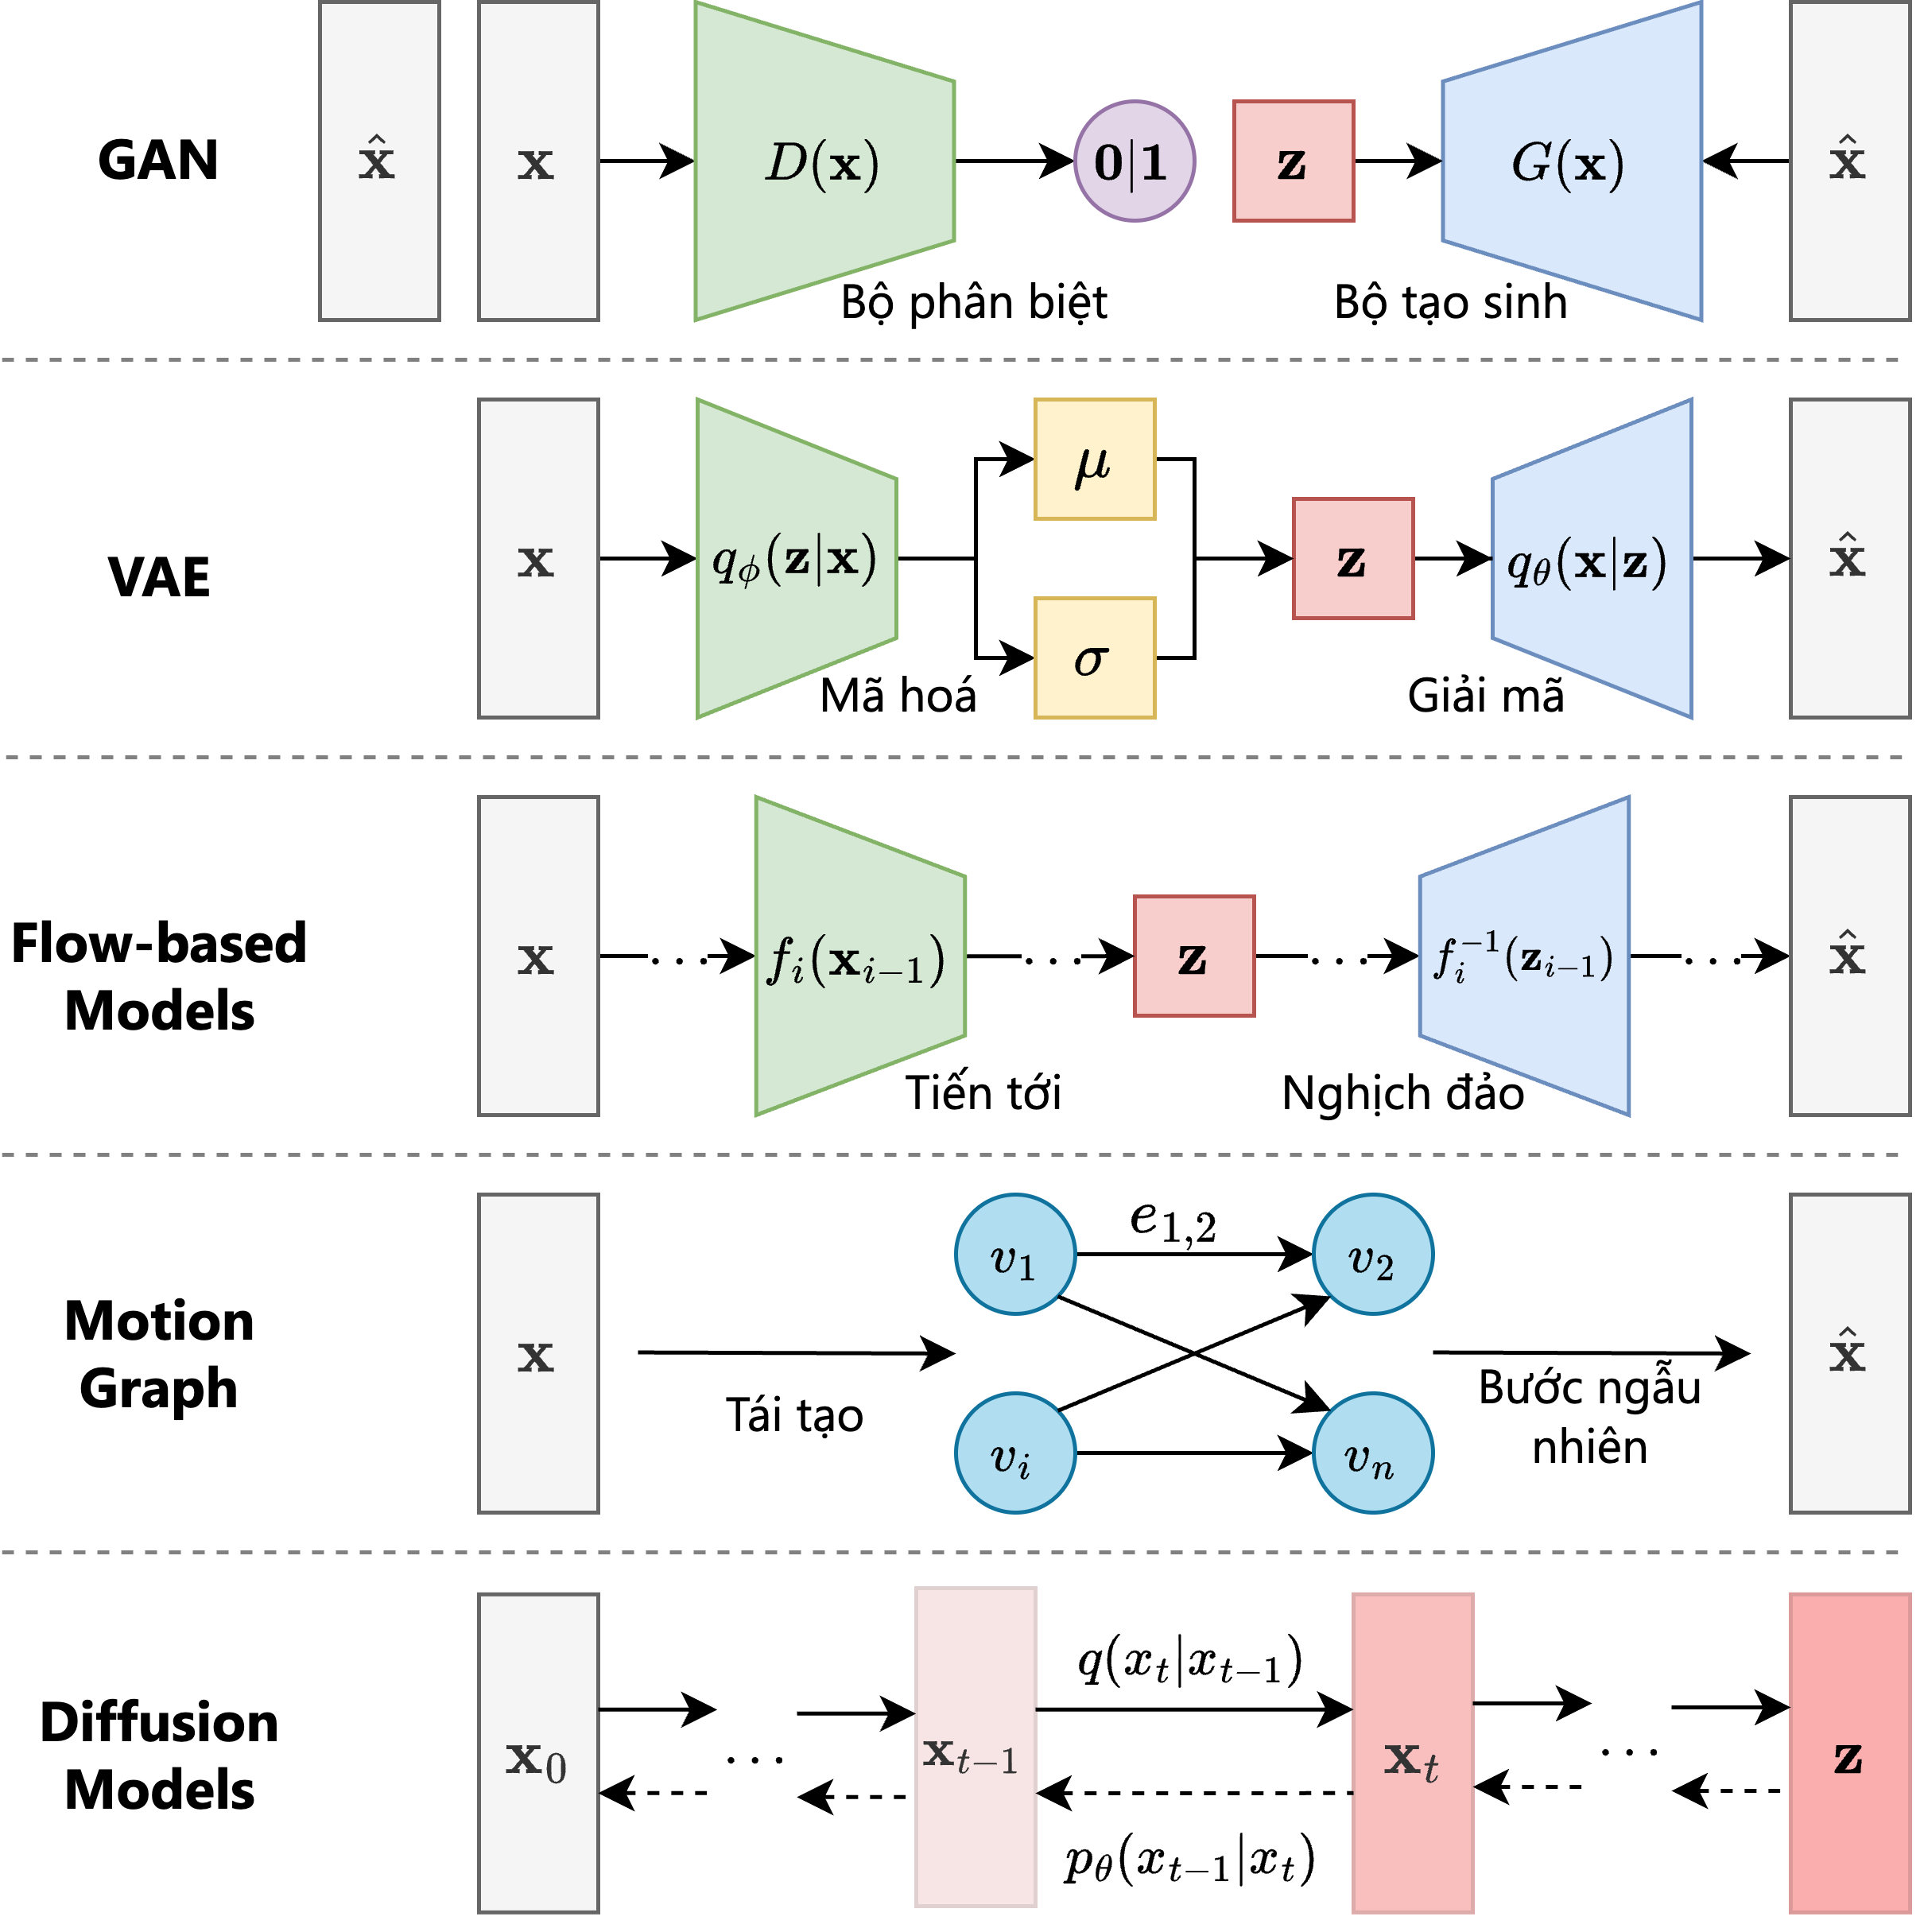
\includegraphics[width=0.8\textwidth]{GeneralOverview}
	\caption{Tổng quan về các mô hình tạo sinh khác nhau.}
	\label{fig:GeneralOverview}
\end{figure}

Phương pháp sinh cử chỉ bằng học sâu minh họa ở \autoref{fig:GeneralOverview} được chia thành hai nhóm chính: học dựa trên ước lượng likelihood (likelihood-based model)  và phương pháp dựa vào các mô hình sinh ngầm định (implicit generative models) \cite{song2021score}.

\subsubsection{Mô hình dựa trên likelihood}

\textbf{Nguyên lý chung của mô hình dựa trên likelihood}

Mô hình dựa trên Likelihood hoạt động bằng cách tối đa hóa xác suất hợp lý của dữ liệu quan sát được, dựa trên các tham số $\theta$ của mô hình. Mục tiêu là tìm được tham số tối ưu $\theta'$ dựa trên xác suất $p(\mathbf{x})$ của dữ liệu, trong đó $\mathbf{x}$ là dữ liệu chuỗi cử chỉ.

\textbf{Phương pháp}

Quá trình áp dụng các phương pháp học sâu vào bài toán sinh cử chỉ cũng tương đồng với sự phát triển của các phương pháp học sâu, từ RNN, LSTM và Transformer .v.v. Các phương pháp tiêu biểu trong nhóm phương pháp dựa trên likelihood:

\begin{itemize}[]
	\item Phương pháp \textit{Gesticulator} \cite{kucherenko2020gesticulator} sử dụng kiến trúc Multilayer Perceptron (MLP) để mã hóa đặc trưng văn bản và âm thanh, sử dụng vector văn bản từ BERT làm vector đặc trưng cho văn bản. 
	
	\item Trong \textit{HA2G} \cite{liu2022learning} dựa trên kiến trúc Transformer xây dựng một mô hình phân cấp (hierarchical) để học các tương quan ở nhiều cấp độ giữa lời nói và cử chỉ, từ các đặc trưng cục bộ (local) đến toàn cục (global). 
	
	\item \textit{Gesture Generation from Trimodal Context} \cite{yoon2020speech} dựa trên kiến trúc RNN, coi việc sinh cử chỉ là bài toán dịch trong xử lý ngôn ngữ. 
	
	\item \textit{DNN} \cite{chiu2015predicting} sử dụng LSTM kết hợp GRU để xây dựng mô hình phân loại (classifier neural network) từng đơn vị cử chỉ để chọn một đơn vị cử chỉ phù hợp dựa trên đầu vào là giọng nói. 
	
	\item \textit{Cascaded Motion Network (CaMN)} \cite{liu2022beat} đề xuất tập dữ liệu BEAT đồng thời đề xuất mô hình giống như thác nước, các thông tin về người nói, nhãn cảm xúc, văn bản, giọng nói và cử chỉ được đi qua các lớp để trích xuất đặc trưng để được các vector tiềm ẩn. Trong giai đoạn kết hợp các đặc trưng, mô hình CaMN kết hợp các đặc trưng theo hình thác nước, lần lượt kết hợp các đặc trưng người nói và cảm xúc, và tiếp tục kết hợp với các vector tiềm ẩn của văn bản, giọng nói và cử chỉ.
	
	\item \textbf{Motion Graph} : Trong phương pháp \textit{Gesturemaster} \cite{zhou2022gesturemaster}, mô hình xây dựng đồ thị ngữ nghĩa, từ trong câu được kết nối trong một đồ thị, nơi các liên kết biểu thị quan hệ ngữ nghĩa giữa chúng. Dựa trên thông tin đồ thị, mô hình chọn các đỉnh (node) và cạnh (edges) có sự tương đồng nhất để biểu diễn cử chỉ. 
	
\end{itemize}

\subsubsection{Mô hình sinh ngầm định}
\label{sec:ImplicitGenerativeModels}

\textbf{Nguyên lý}

Mô hình sinh ngầm định học phân phối dữ liệu mà không cần biểu diễn tường minh hàm mật độ xác suất $p(\bx)$. Thay vì trực tiếp tính xác suất $p(\bx)$, mô hình sẽ học một ánh xạ $G_{\theta}: \mathcal{Z} \to \mathcal{X}$ thông qua so khớp phân phối giữa dữ liệu thật và dữ liệu sinh ra $\mathbf{x} = G_\theta(\mathbf{z}), \quad \mathbf{z} \sim p_z(\mathbf{z})$.  Trong đó $\mathcal{Z}$ là không gian nhiễu đầu vào, thường có phân phối đơn giản \(p_{z}\) (ví dụ: Gaussian, Uniform). \(\mathcal{X}\) là không gian dữ liệu thực, là chuỗi cử chỉ \(\mathbf{x}\). 

Trong bài toán sinh cử chỉ, để kết hợp thêm các điều kiện về giọng nói, nhãn văn bản, các mô hình sinh ngầm định thường kết hợp thêm điều kiện $\mathbf{c}$, với điều kiện là ngữ cảnh của bài toán để có được kết quả sinh: $\mathbf{x} = G_\theta(\mathbf{z}, \mathbf{c})$. Ngữ cảnh của bài toán có thể bao gồm giọng nói, văn bản, mã định danh người nói, phong cách, cảm xúc hay cử chỉ khởi tạo.

%
Ví dụ tiêu biểu nhất là mô hình generative adversarial networks (GANs) và Diffusion. Khi dữ liệu được tổng hợp bằng cách chuyển phân phối dữ liệu ban đầu ở dạng phân phối chuẩn về phân phối của dữ liệu.

\textbf{Phương pháp} 

Các phương pháp tiêu biểu cho mô hình sinh ngầm định là 

\begin{itemize}
	\item \textit{MoGlow} \cite{henter2020moglow} sử dụng Normalizing Flows được sử dụng để duy trì tính nhất quán và tính tương thích của chuyển động, đồng thời cung cấp khả năng điều khiển thông qua các thông số đầu vào. Điều này cho phép người dùng tạo ra các chuyển động mới hoặc thay đổi các chuyển động hiện có bằng cách thay đổi các thông số điều khiển.
	
	\item \textbf{GAN}: \textit{GRU-based WGAN} \cite{wu2021probabilistic} sử dụng Wasserstein GAN để đánh giá và cải thiện chất lượng của việc sinh cử chỉ, mô hình tập trung vào việc tối ưu hóa hàm mất mát Wasserstein, giúp giảm tình trạng chảy đặc (mode collapse) thường gặp trong GAN truyền thống. GRU được sử dụng để xử lý dữ liệu lời nói và biến nó thành các đặc trưng cử chỉ có thể sử dụng được. Sau đó, những đặc trưng này được cung cấp vào mạng WGAN, nơi chúng sẽ được đánh giá và tinh chỉnh để sinh cử chỉ.
	
	\item \textbf{VAE}:  \textit{FreeMo} \cite{xu2022freeform} sử dụng VAE để phân rã (decomposing) các cử chỉ thành tư thế cử chỉ (pose modes) và giai điệu chuyển động (rhythmic motions). Tư thế cử chỉ được sinh ra ngẫu nhiên sử dụng quá trình lấy mẫu có điều kiện trong không gian ẩn của VAE. Trong khi các giai điệu chuyển động được sinh ra từ 
	
	\item \textbf{VQ-VAE} \textit{Rhythmic Gesticulator} \cite{ao2022rhythmic} tiền xử lý các đoạn giọng nói theo nhịp điệu (beats) để tách giọng nói thành các đoạn nhỏ, và biểu diễn chúng thành các khối theo kích thước chuẩn hóa (normalization). Tương tự phương pháp VQ-VAE, các chuỗi cử chỉ đã chuẩn hóa sẽ được lượng tử hóa (quantization) thành các vùng không gian khác nhau của cử chỉ được gọi là các từ vựng cử chỉ (gesture lexicon). Mô hình học từ vựng cử chỉ (gesture lexicon) từ khối chuẩn hóa trên với điều kiện là cử chỉ trước đó, phong cách cử chỉ và giọng nói. Sau đó mô hình tái tạo lại từ quá trình chuẩn hóa (denormalization) để có được chuỗi cử chỉ ban đầu. Khác với mô hình sinh ngầm định như GANs hay Diffusion, VQ-VAE thường tập trung vào việc nén dữ liệu hơn là sinh dữ liệu trực tiếp.
	
	\item \textbf{Diffusion}:  Mô hình Diffusion tập trung vào việc tạo ra dữ liệu mới từ trạng thái nhiễu, phục hồi ngược lại dữ liệu gốc. Các phương pháp dựa trên Diffusion sẽ được trình bày ở mục \autoref{sec:diffusionbase}
	
\end{itemize}


\subsection{So sánh các phương pháp sinh cử chỉ}

\begin{table}[H]
	\small
	\centering
	\renewcommand{\arraystretch}{1.5} % Tăng khoảng cách giữa các hàng
	\resizebox{\textwidth}{!}{ % Giảm kích thước bảng để vừa với trang
		\begin{tabular}{|p{0.2\textwidth}|p{0.35\textwidth}|p{0.35\textwidth}|p{0.2\textwidth}|}
			\hline
			\textbf{Phương pháp tiêu biểu} & \textbf{Ưu điểm} & \textbf{Nhược điểm} & \textbf{Loại phương pháp} \\ \hline
			Robot behavior toolkit \cite{huang2012robot} & 
			- Dễ hiểu và dễ triển khai. \newline 
			- Dễ giải thích và có thể kiểm soát được \newline
			- Hiệu quả trong các trường hợp đơn giản hoặc dữ liệu nhỏ. & 
			- Không tổng quát hóa tốt với dữ liệu phức tạp. \newline 
			- Đòi hỏi nhiều công sức trong việc xây dựng quy tắc thủ công. & 
			Mô hình dựa trên luật  \\ \hline
			MLP \cite{kucherenko2020gesticulator}, RNN \cite{bhattacharya2021speech2affectivegestures}, \cite{liu2022learning}, \cite{hasegawa2018evaluation}, \cite{yoon2020speech}, CNN \cite{habibie2021learning}, Transformer \cite{bhattacharya2021text2gestures}  & 
			- Khả năng ước lượng mật độ xác suất của dữ liệu \newline 
			- Có khả năng mở rộng và học từ dữ liệu lớn & 
			- Dễ bị ảnh hưởng bởi nhiễu \newline 
			- Kết quả thấp ở vùng dữ liệu hiếm \newline
			- Khả năng sinh không đa dạng & 
			Mô hình dựa trên Likelihood \\ \hline
			\textbf{DiffusionStyle-Gesture} \cite{yang2023diffusestylegesture}, MDM \cite{tevet2022human}, Motiondiffuse \cite{zhang2022motiondiffuse} &
			- Tạo ra dữ liệu chất lượng cao. \newline 
			- Linh hoạt và đa dạng \newline
			- Phủ được vùng có mật độ dữ liệu thấp & 
			- Cần cấu hình phức tạp để đạt hiệu năng tốt. \newline 
			- Mỗi lần lấy nhiễu ngẫu nhiên là khác nhau. \newline 
			- Quá trình lấy mẫu chậm & 
			Mô hình sinh ngầm định\\ \hline
		\end{tabular}
	}
	\caption{Bảng so sánh ưu và nhược điểm của các phương pháp}
	\label{table:CompareMethod}
\end{table}

%\textbf{Bảng so sánh các phương pháp}
%
%\begin{table}[ht]
%	\centering
%	\begin{tabular}{|l|l|l|l|l|l|}
%		\hline
%		\textbf{Phương pháp} & \textbf{Loại mô hình} & \textbf{Đặc điểm nổi bật} & \textbf{Ưu điểm} & \textbf{Hạn chế} & \textbf{Tài liệu tham khảo} \\ \hline
%		VAE  & Autoencoder & Biểu diễn dữ liệu trong không gian tiềm ẩn & Tạo đặc trưng ẩn & Khó kiểm soát đầu ra & \cite{kingma2013auto} \\ \hline
%		VQ-VAE & Autoencoder (cải tiến) & Dùng codebook cho không gian tiềm ẩn & Biểu diễn chi tiết hơn & Phức tạp hơn & \cite{van2017neural} \\ \hline
%		RNN & Mạng hồi tiếp & Xử lý chuỗi dữ liệu & Tốt cho dữ liệu tuần tự & Khó huấn luyện & \cite{bhattacharya2021speech2affectivegestures} \\ \hline
%		Transformer & Mạng chú ý & Tạo cử chỉ qua cơ chế chú ý & Hiệu quả với dữ liệu dài & Yêu cầu nhiều tài nguyên & \cite{bhattacharya2021text2gestures} \\ \hline
%		WGAN & GAN & Học phân phối dữ liệu đối kháng & Tạo sự đa dạng & Khó huấn luyện & \cite{wu2021probabilistic} \\ \hline
%		Normalizing Flow & Mô hình xác suất & Học phân phối phức tạp & Hữu ích với dữ liệu phức tạp & Cần tài nguyên tính toán lớn & \cite{alexanderson2020style} \\ \hline
%		Diffusion Models & Mô hình sinh dữ liệu & Chi tiết cao, xử lý dữ liệu thiếu & Tạo cử chỉ chi tiết & Thời gian huấn luyện lâu & \cite{xu2022freeform} \\ \hline
%	\end{tabular}
%	\caption{So sánh các phương pháp sinh cử chỉ}
%\end{table}
